\documentclass[11pt]{article}
\usepackage{amsmath,flexisym,textcomp,amssymb,geometry,graphicx,enumerate}

\def\Name{Quoc Thai Nguyen Truong}  % Your name
\def\SID{24547327}  % Your student ID number
\def\Login{cs170-ig} % Your login (your class account, cs170-xy)
\def\Homework{6}%Number of Homework
\def\Session{Fall 2014}


\title{CS170--Fall 2014 --- Solutions to Homework \Homework}
\author{\Name, SID \SID, \texttt{\Login}}
\markboth{CS170--\Session\  Homework \Homework\ \Name}{CS170--\Session\ Homework \Homework\ \Name, \texttt{\Login}}
\pagestyle{myheadings}

\newcommand{\tab}{\hspace*{2em}}

\newenvironment{qparts}{\begin{enumerate}[{(}a{)}]}{\end{enumerate}}
\def\endproofmark{$\Box$}
\newenvironment{proof}{\par{\bf Proof}:}{\endproofmark\smallskip}

\textheight=9in
\textwidth=6.5in
\topmargin=-.75in
\oddsidemargin=0.25in
\evensidemargin=0.25in


\begin{document}
\maketitle

\noindent
Collaborators: Brian Chu

\section*{1. Fundamental concepts}
\begin{qparts}
\item
True.\\
If there if an edge between $v_i\ and\ v_j$ and $v_i\ is\ point\ to\ v_j$. Therefore, in the Topologically sorted, $v_i$ must come before $v_j$, and topologically sorted guaranteed to have $v_i$ before $v_j$ in the list.
\item
True\\
We know G is a DAG. If there if an path from $v_i\ to\ v_j$ so that $v_i\ to\ v_{i+1}\ to \cdots\ to  v_j$. Therefore, in the Topologically sorted, $v_i$ must come before $v_{i+1}$, and so on. Hence, $v_i$ must come before  $v_j$ and topologically sorted guaranteed to have $v_i$ before $v_j$ in the list.
\item
False\\
Counter example : If G has 2 cycles, u is in 1 cycle and v is in other cycle, and there is an edge (u,v) in G. Hence, u is in SSC in its cycle, and v is in other SSC in its cycle. However, u and v are not in the same strongly connected component.
\item
False\\
Counter example : $S\to B\longleftarrow A\longrightarrow t$. We can see that there is no path from s to t.

\item
False\\
Counter example: Let G has n vertices $(n>3)$, and v be a vertex in G. If every other vertices are point to v, and v must have at most $(n-1)$ incoming edges which more than 3.
\item
False\\
Counter example: Let G has n vertices, and v be a source node in G. If v point to every other $(n-1)$, then there are at most $(n-1)!$ possible ways to order the vertices so they are in topologically sorted order.

\item
False\\
Counter example:\\
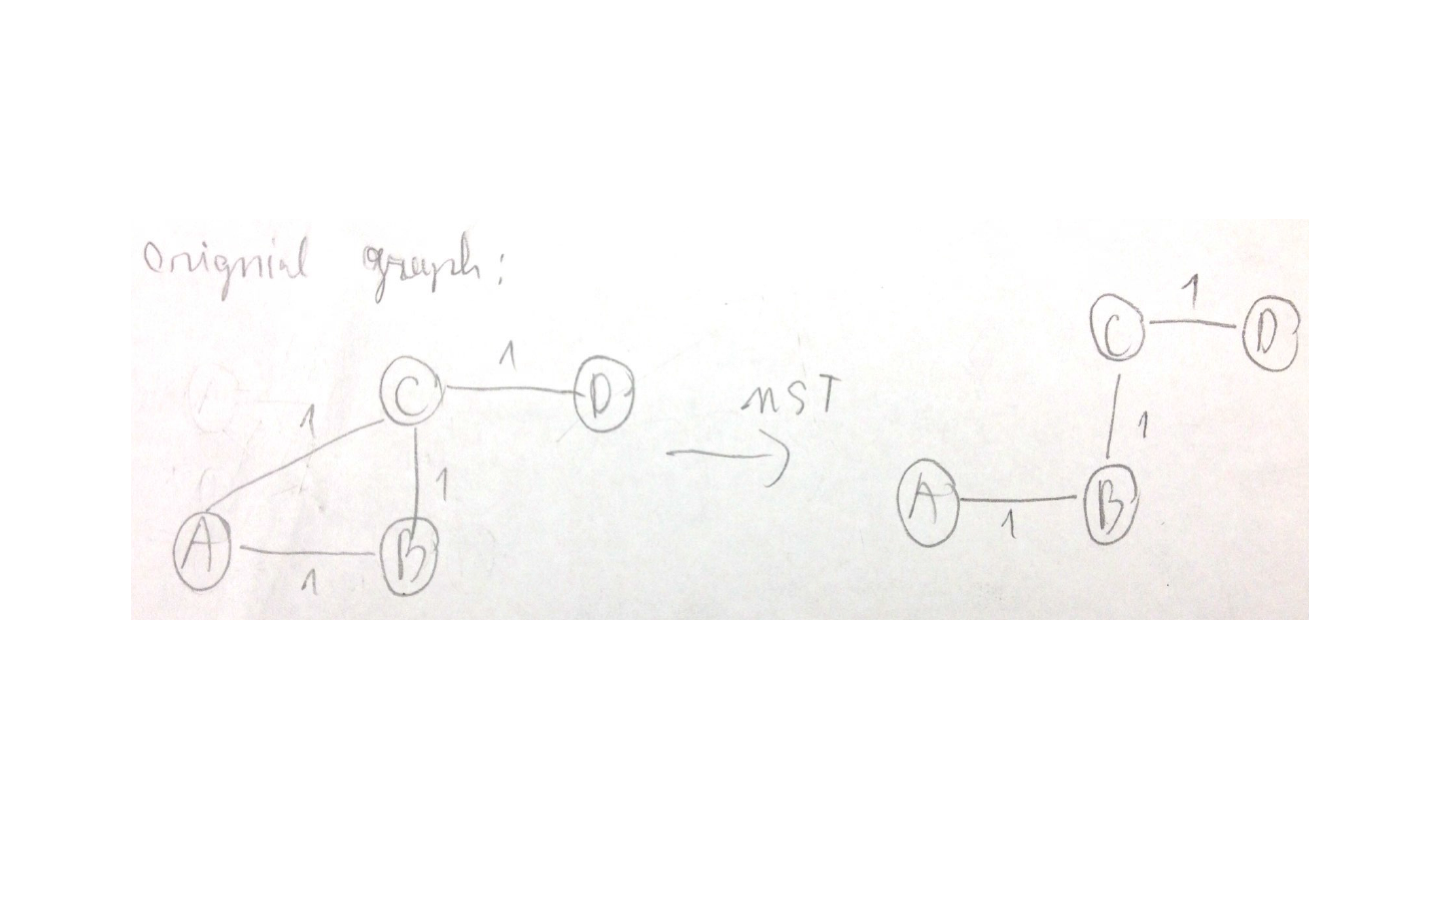
\includegraphics[scale=0.25]{p1g.png}\\
In the picture above, 1 is the smallest length for every edges in the graph, and there is only one possible minimum spanning tree of the graph.However, the edge (A,C) is not in the minimum spanning tree. Therefore, the answer is False.
\item
True\\
The different thing from 1g is that there exist a minimum length in the graph. Therefore the edge with minimum length will be in every minimum spanning tree of G.\\
\end{qparts}



% You can include a picture using the following:
%   \begin{center}
%   \includegraphics[scale=1]{picturefile.pdf}
%   \end{center}
% (remove the percent signs at the start of the lines above)
% you can also use a .png image, but other file formats are alas
% not supported by Latex.


\newpage
\section*{2. BFS?}
This is $\boxed{NOT}$ guaranteed to produce a valid topological sorting of the vertices.\\
Counter Example:\\
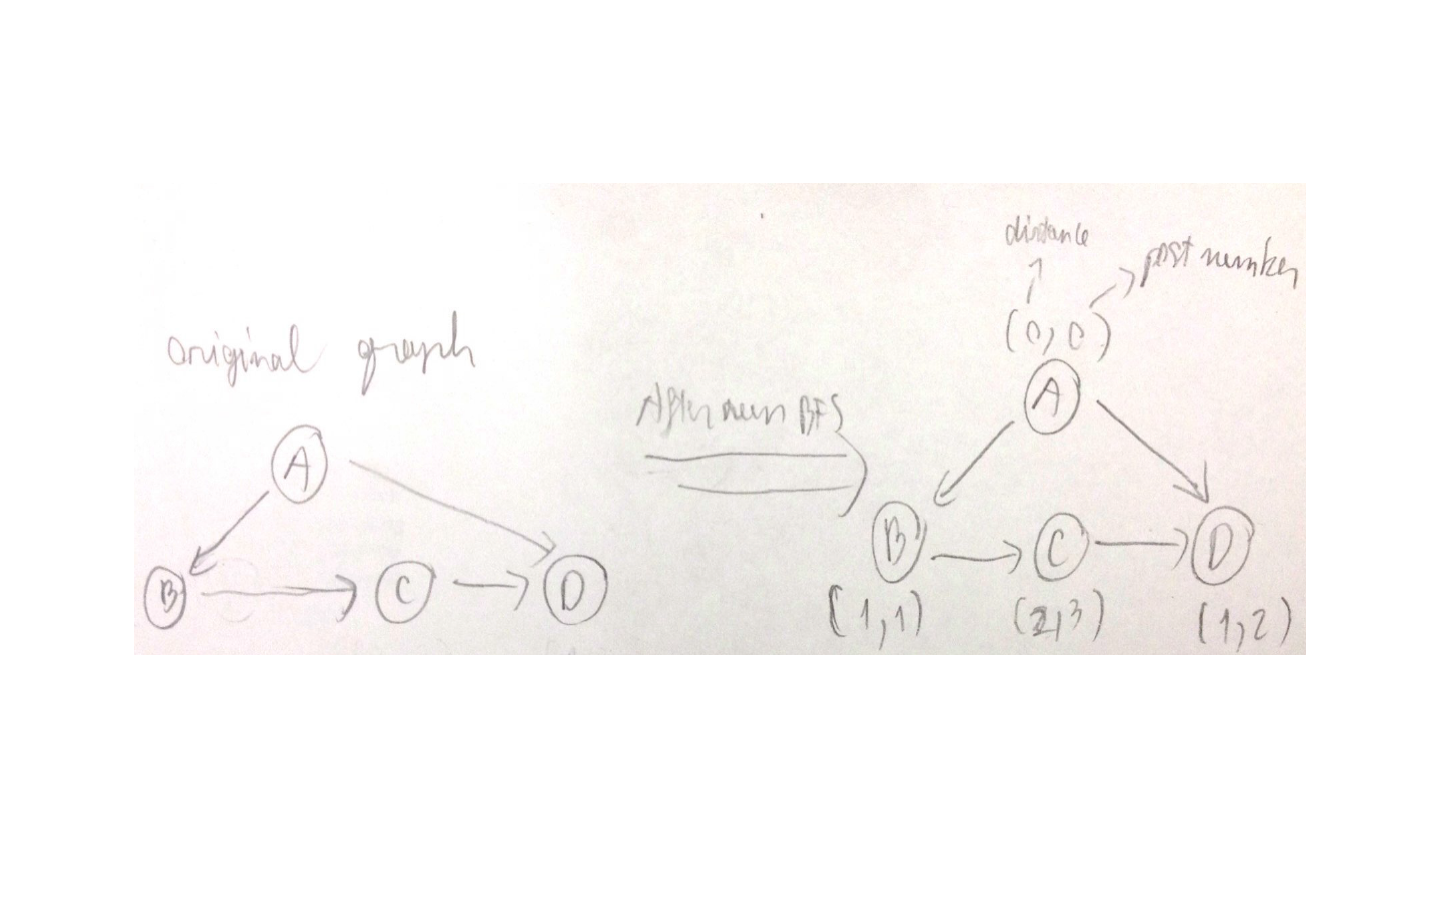
\includegraphics[scale=0.3]{p2.png}\\
In the picture, we can see that sorting by increasing post-value by running BFS will give us [A,B,D,C] which is not the same as it suppose to be as [A,B,C,D]

\newpage
\section*{3. Travel planning}
\noindent
\textbf{Main idea.}\\
The idea is to add $\frac{1}{n}$ to length of every edge, and run Dijkstra on the graph. If there are paths that has the same cost from city A to city B and different number of fight, adding an addition cost of $\frac{1}{n}$ will make cost of the path that has greater number of flights be greater than the path that has less number of flights. Hence, we run Dijkstra on the graph with new edges cost, and get the path from city A to city B with the minimum cost and minimum number of fights.


\noindent
\textbf{Pseudocode.}\\
Line 0: Travel(graph G):\\
Line 1: path = []\\
Line 2: For every edge e in edge E in G:\\
Line 3:\tab cost(e) = cost(e) + $\frac{1}{n}$ \# n is number of cities is also the number vertices.\\
Line 4: path = Dijkstra(city A, city B)\\
Line 5: return path\\


\noindent
\textbf{Proof of correctness.}
\_ Direct Proof:\\
If there exist multiple shortest paths which has the same cost but different number of flights (vertices) from city A to city B. Adding cost of $\frac{1}{n}$ to each edge will crease the cost of all the path. Obviously, we can see that the cost of the paths has more flights (vertices) is bigger than the total cost of the paths has less flights (vertices). Hence, running Dijkstra will guarantee to get the shortest path with the minimum of flights. Therefore, the algorithm works\\


\noindent
\textbf{Running time.}
$$\boxed{T(n) = \Theta(n^2)\log(n)}$$

\noindent
\textbf{Justification of running time.}
Let T(n) be the run time for the algorithm, with n is number of cities.\\
Assume that we have the max edges of $\frac{n(n-1)}{2}$\\
At line 2 and 3, adding all the edges will take $\Theta(n^2)$\\
At line 4 run Dijkstra will take $\Theta(n^2 + n)\log(n)$\\
Therefore,
$$T(n) = \Theta(n^2) + \Theta(n^2 + n)\log(n) = \Theta(n^2)\log(n)$$

\newpage
\section*{4. Road network design}
\noindent
\textbf{Main idea.}\\
The idea is to make 2 copies of graph G (Copy1 has vertices $s_1$ and $t_1$, and Copy2 has vertices $s_2$ and $t_2$). Then connect all candidates roads from graph Copy1 to  graph Copy2. After that, run Dijkstra($s_1$, $t_2$), to get the shortest path  from $s_1$ to $t_2$,and we know that it contains only 1 candidate. Hence, when running Dijkstra, it should store the candidate road which is the pair of cities ($a_i,b_i$), and we return the index i in pair that pair.\\
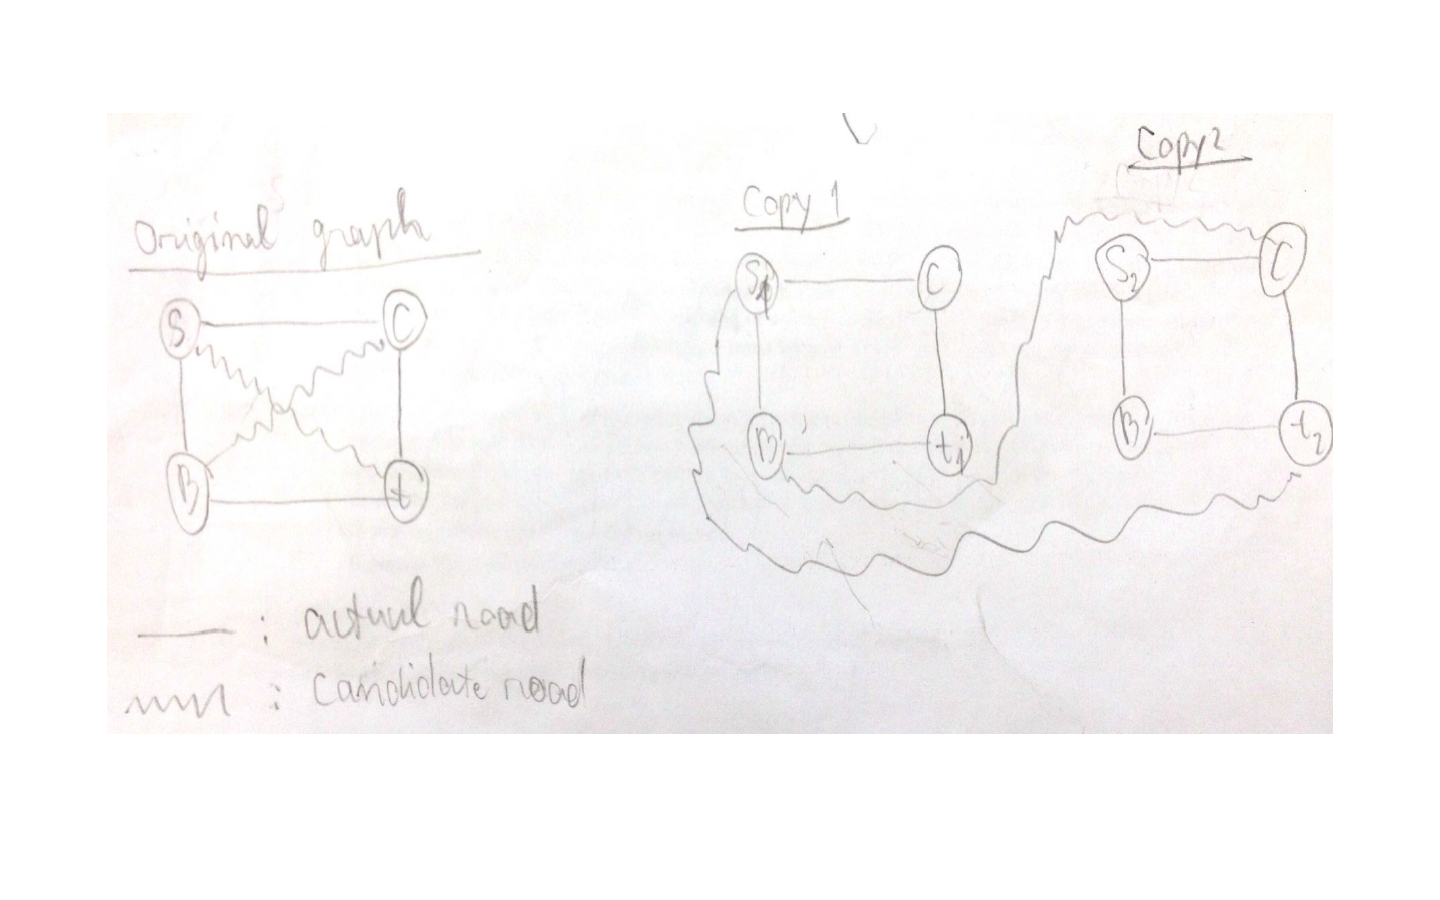
\includegraphics[scale=0.25]{p4.png}\\

\noindent
\textbf{Pseudocode.}\\
Line 0: Function(graph G, s,t, candidates roads $[(a_1,b_1),\cdots,(a_n,b_n)]$):\\
Line 1:\tab Copy1 = make a copy of graph G (vertices $s_1$ and $t_1$) (no candidates roads) \\
Line 2:\tab Copy2 = make a copy of graph G (vertices $s_2$ and $t_2$) (no candidates roads)\\
Line 3:\tab Y = connected all candidates roads $(a_i,b_i)$ $( 0\leqslant i\leqslant n)$, for $a_i$ is vertex in Copy1 and $b_i$ is vertex in Copy2\\
Line 4:\tab shortestPath = Dijkstra(graph Y,$s_1$,$t_2$)\\
Line 5:\tab For each edge e in shortestPath:\\
Line 6:\tab\tab If e in candidates roads $[(a_1,b_1),\cdots,(a_n,b_n)]$:\\
Line 7:\tab\tab\tab return index of candidates roads\\

\noindent
\textbf{Proof of correctness.}\\
Running Dijkstra from the start vertex $s_1$ of graph Copy1 to the goal vertex $t_2$ of graph Copy2, then the solution for the shortest path must be : $s_1, i, j,\cdots, t_2$. In order to go from graph Copy1 to the graph Copy2 , it must take one candidate road to go from Copy1 to graph Copy2. Hence, the shortest path must contain at least one candidate road. We know that graph Copy1 and graph Copy2 has exactly the same cost of each edges (since they're copy of the original graph without candidate road). Therefore, shortest path that Dijkstra return must have exactly one candidates road and the path should have a format of [edges in graph Copy1, one candidate road, edges in graph Copy2] which is $[s_1,\cdots, a_i,b_i, \cdots, t_2]$. Therefore, the algorithm works.\\

\noindent
\textbf{Running time.}
$$\boxed{T(E,V) = \Theta((|E| + |V|)\log(V))}$$

\noindent
\textbf{Justification of running time.}
Let T(E,V) be the run time of the algorithm, with V vertices and E edges in graph G.\\
From the Piazza post, a GSI "Baruch Sterin" told us that we can assume $n = \Theta(|V| + |E|)$\\
\\
At line 3 and 4, make a copy of Graph G will take $\Theta(|E| + |V|)$\\
At line 5, connected all candidates roads between 2 copy graphs will take $\Theta(|E| + |V|)$\\
At line 6, run ModifiedDijkstra will take $\Theta((|E| + |V|)\log(n))$\\
Therefore,
$$T(E,V) = \Theta(|V| + |E|) + \Theta(|V| + |E|) + \Theta((|E| + |V|)\log(V)) = \Theta((|E| + |V|)\log(V))$$ 




\newpage
\section*{5. MSTs for directed graphs}
We are $\boxed{NOT}$ guarantee that $G^*$ has the minimal possible total weight, out of all possible graphs $G\textprime$ = $(V,E\textprime)$ such that $E\textprime \subseteq E$ and $G\textprime$ is strongly connected\\
Counter Example:\\
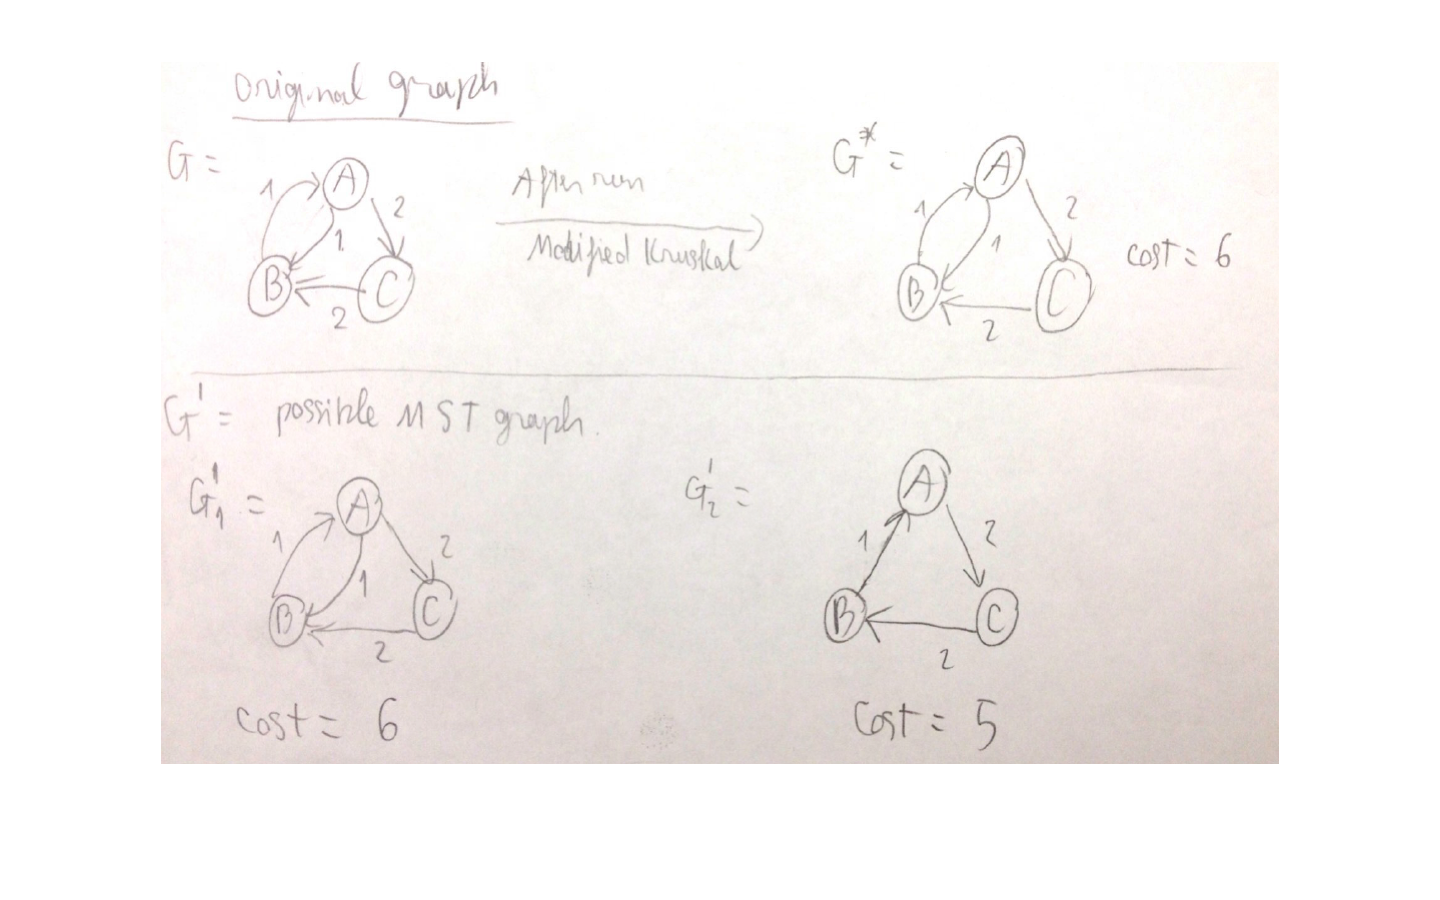
\includegraphics[scale=0.3]{p5.png}\\
In the picture above, we can see that after running ModifiedKruskal, $G\textprime$ is the same as $G$ which has the cost of 6. However,$G\textprime$ (in picture above) has 2 possible graph $G_1\textprime$ and $G_2\textprime$. $G_2\textprime$ has the cost of 5 which is less than 6 the cost  of $G^*$. This is saying that $G^*$ is not the minimal possible total weight out of all possible graph $G\textprime$. Therefore, the answer is NO.



% Tempted to submit a solution for Q6?
% (Crazy hard optional problem: Two vertex-disjoint paths)
% Don't bother - we won't grade it.

\end{document}
